% MLST submission build: run `make submission` in paper/ to produce
% main_submission.pdf (12 pt single column, per IOP's review-format preference).
\documentclass[aps,prd,twocolumn,superscriptaddress,nofootinbib]{revtex4-2}

\usepackage{amsmath,amssymb}
\usepackage{graphicx}
\usepackage{hyperref}
\usepackage{xcolor}
\usepackage{booktabs}
\usepackage{multirow}
\usepackage{tikz}
\usetikzlibrary{positioning,arrows.meta,decorations.pathreplacing,calc}

% Custom commands
\newcommand{\phifour}{\ensuremath{\phi^4}}
\newcommand{\SE}{\ensuremath{S_E}}
\newcommand{\xiL}{\ensuremath{\xi/L}}
\newcommand{\msq}{\ensuremath{m^2}}
\newcommand{\msqc}{\ensuremath{m^2_c}}
\newcommand{\pyg}{\textsc{PyG}}
\newcommand{\todo}[1]{\textcolor{red}{[TODO: #1]}}

% Finite-size-scaling numbers, auto-generated from the cluster analysis by
% scripts/make_fss_numbers.py (ground rule 4). Re-run that script to update.
% Auto-generated by scripts/make_fss_numbers.py -- DO NOT EDIT BY HAND.
% Every FSS number in the paper traces to results/fss_analysis_cluster.json.
\newcommand{\ClGammaNu}{1.732(8)}
\newcommand{\ClGammaNuCorr}{1.720(16)}
\newcommand{\ClGammaNuAIC}{1.731(16)}
\newcommand{\ClNu}{1.04(8)}
\newcommand{\ClMsqc}{-2.217(3)}
\newcommand{\ClNuChiDof}{1.6}
\newcommand{\LocGammaNu}{1.60(3)}
\newcommand{\LocNu}{1.0(5)}
\newcommand{\Nsizes}{7}
\newcommand{\Lmax}{128}
\newcommand{\LocEffSlopeLo}{1.64}
\newcommand{\LocEffSlopeHi}{1.42}
\newcommand{\TauLocLo}{65}
\newcommand{\TauLocHi}{185}
\newcommand{\TauClTyp}{8\text{--}9}
\newcommand{\SpeedupHi}{21}


% Double-anonymous review build: `make anonymous` (in paper/) flips the switch
% below to \anonymoustrue and produces main_anonymous.pdf per the IOP checklist
% (publishingsupport.iopscience.iop.org/questions/checklist-for-anonymising-your-manuscript/).
% Upload the anonymous PDF only -- this .tex retains identity in \else branches.
\newif\ifanonymous
\anonymousfalse
\ifanonymous
\hypersetup{pdfauthor={Anonymous},
  pdftitle={Heterogeneous Bipartite Graph Neural Networks for Lattice Quantum Field Theory}}
\fi

\begin{document}

\title{Heterogeneous Bipartite Graph Neural Networks\\for Lattice Quantum Field Theory}

\ifanonymous
\author{Anonymous}
\affiliation{Author details withheld for double-anonymous review}
\else
\author{Joshua Paul Brehm}
\email{joshua.paul.brehm@gmail.com}
\affiliation{Independent Researcher}
\fi

\date{\today}

\begin{abstract}
We introduce a heterogeneous bipartite graph neural network (GNN) architecture that
separates \emph{spacetime geometry} from \emph{field content} into distinct node
types connected by typed edges---a design inspired by the geometry--matter
distinction in continuum quantum field theory. Unlike existing approaches that
embed all information on spacetime nodes in a homogeneous graph, our
architecture represents fields as a separate layer coupled to the lattice
through typed ``inhabits'' edges and three-stage message passing. We benchmark on
two-dimensional scalar $\phifour$ theory in the Ising universality class ($\nu =
1$), comparing against homogeneous GNN, convolutional, and multilayer-perceptron (MLP) baselines. We show that
homogeneous GNN representations suffer a structural failure mode---message
passing destroys the field signal without ad hoc skip connections---which the
bipartite design eliminates by construction. The model achieves near-perfect action prediction across lattice sizes
($r > 0.9999$ at $8 \times 8$ and $16 \times 16$; median $r = 0.9992$ at
$64 \times 64$), and a single model trained at $16 \times 16$ transfers to
lattices from $8 \times 8$ to $64 \times 64$ with $r = 1.0000$ and no
retraining. The underlying Monte Carlo pipeline reproduces Ising-class
finite-size scaling---order-parameter S-curves, susceptibility-peak growth with
$\gamma/\nu = \ClGammaNu$, and correlation-length crossings giving $\nu = \ClNu$,
consistent with the exact Ising values, once a cluster sampler controls the
critical slowing down of local updates---validating the training distributions. The bipartite
structure naturally accommodates multiple field types (scalar, gauge, fermion) at
the same lattice site, providing a direct path to gauge theories and lattice
quantum chromodynamics (QCD) without architectural changes.
\end{abstract}

% Keywords for the MLST submission form (revtex4-2/prd does not render them):
% graph neural networks; lattice field theory; heterogeneous graphs;
% action matching; Monte Carlo simulation; finite-size scaling;
% critical exponents; machine learning for physics
%
% Social media abstract for the MLST submission form (95 chars, limit 100):
% A #GNN that separates spacetime from matter learns lattice φ⁴ theory and transfers across sizes

\maketitle

%=============================================================================
\section{Introduction}
\label{sec:intro}
%=============================================================================

Lattice quantum field theory is the primary non-perturbative tool for studying
strongly coupled quantum systems, underpinning our quantitative understanding of
hadron physics through lattice quantum chromodynamics (QCD)~\cite{Wilson1974}. Despite decades of
algorithmic advances, lattice calculations face persistent computational
bottlenecks: critical slowing down near phase transitions, the fermion sign
problem at finite baryon density, and the inability to directly simulate
real-time dynamics in Minkowski spacetime.

Machine learning methods have shown promise in addressing several of these
challenges. Normalizing flows can accelerate sampling by learning the Boltzmann
distribution~\cite{Kanwar2020,Boyda2021}, while neural networks can learn
lattice observables directly from field configurations---via gauge-equivariant
convolutional architectures~\cite{Favoni2022} or graph neural networks
(GNNs)~\cite{Bachtis2021}. However, existing GNN approaches
treat the lattice as a \emph{homogeneous graph}, embedding field values (scalar,
gauge links, spinor components) as features on spacetime nodes. This conflates
two fundamentally different objects: the geometry of spacetime and the dynamical
content of quantum fields.

In continuum QFT, the action functional separates geometry from matter:
\begin{equation}
S[\phi, g] = \int d^dx\, \sqrt{g}\, \Big[\tfrac{1}{2} g^{\mu\nu} \partial_\mu\phi\, \partial_\nu\phi + V(\phi)\Big],
\label{eq:continuum-action}
\end{equation}
where the metric $g_{\mu\nu}$ encodes spacetime geometry and $\phi$ encodes
field content. These couple through the action but are distinct mathematical
objects living in different spaces.

We propose a \emph{heterogeneous bipartite graph} architecture built around this
separation on the lattice. Spacetime nodes encode lattice geometry
(coordinates, spacing, boundary conditions), while field nodes encode dynamical
degrees of freedom (scalar values, gauge link matrices, spinor components). The
two layers communicate through typed ``inhabits'' edges and three-stage message
passing. This design has several advantages:

\begin{enumerate}
\item \textbf{Natural multi-field handling:} Multiple field types at the same
site are distinct nodes with separate encoders, avoiding feature concatenation.
\item \textbf{Dynamic geometry:} Spacetime node positions can be made learnable,
enabling adaptive mesh refinement.
\item \textbf{Extensibility:} Adding gauge or fermion fields requires only new
encoder modules, not architectural changes.
\item \textbf{Physical interpretability:} The bipartite structure preserves the
geometry--matter distinction through the entire network.
\end{enumerate}

We benchmark this architecture on two-dimensional scalar $\phifour$ theory, the
simplest interacting field theory with a well-understood phase transition in the
Ising universality class ($\nu = 1$ exactly). This provides a rigorous test:
the model must learn the action functional, reproduce the phase transition, and
yield correct finite-size scaling across lattice sizes up to $L = \Lmax$.

\subsection{Related Work and Novelty}
\label{sec:related}

Machine learning approaches to lattice field theory have developed along several
directions (see Ref.~\cite{Cranmer2023} for a recent review). Normalizing flows
learn the Boltzmann distribution for efficient
sampling~\cite{Albergo2019,Kanwar2020,Boyda2021}. Gauge-equivariant and
gauge-invariant neural networks enforce exact lattice symmetries in the network
architecture~\cite{Favoni2022,Luo2021,Apte2024}. Graph neural networks have been
applied to learn field-theoretic observables~\cite{Bachtis2021}, and relational
inductive biases have proven valuable in broader physics
contexts~\cite{Cranmer2020,Battaglia2018}. In the machine-learning literature,
heterogeneous graphs with typed nodes and relations are a well-developed
modeling tool~\cite{Schlichtkrull2018,Hu2020}, but to our knowledge they have
not been applied to the geometry--field decomposition of lattice field theory.

These approaches share a common representation: field variables are attached
directly to lattice sites or links, with all information embedded on a single
node type in a homogeneous graph (or equivalently on a regular grid). While
effective, this conflates spacetime geometry with field content---objects that
are mathematically distinct in continuum QFT.

Our contribution is a \emph{heterogeneous bipartite graph formulation} in which
spacetime geometry and field degrees of freedom are represented as distinct node
types connected by typed edges. This structure is loosely analogous to a fiber
bundle: spacetime nodes play the role of the discrete base manifold $M$, each
field node represents a point in the fiber over its site (so that a field
configuration --- the collection of all field-node values --- is a discretized
section), and the ``inhabits'' edges encode the projection $\pi: E \to M$
associating each field value to its spacetime site. The three-stage message-passing protocol
(field~$\to$~spacetime, spacetime~$\to$~spacetime, spacetime~$\to$~field) acts
as a discrete analog of the field--geometry coupling encoded in the action
functional. The resulting architecture naturally supports multiple field
types at a single lattice site without feature concatenation and provides a
modular pathway to more complex theories, including gauge fields and fermions.

%=============================================================================
\section{Architecture}
\label{sec:architecture}
%=============================================================================

\subsection{Heterogeneous Bipartite Graph}
\label{sec:graph-structure}

For a scalar field theory on an $L \times L$ lattice with periodic boundary
conditions, the graph $\mathcal{G} = (\mathcal{V}, \mathcal{E})$ consists of
two node types and three edge types:

\begin{figure}[t]
\centering
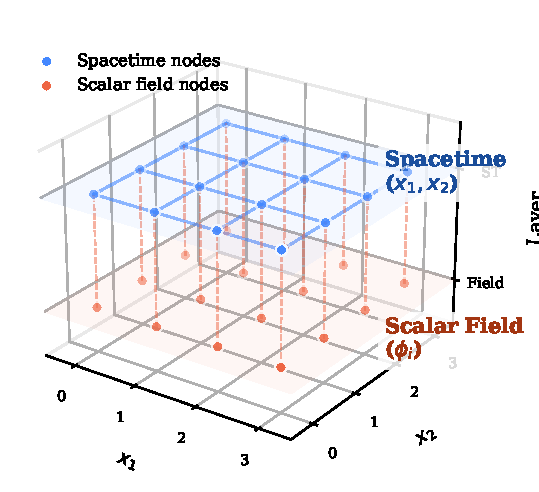
\includegraphics[width=\columnwidth]{figures/graph_structure.pdf}
\caption{3D view of the heterogeneous bipartite graph for a $4\times 4$ lattice.
Blue spheres (upper plane): spacetime nodes with coordinate features $(x_1, x_2)$.
Orange spheres (lower plane): scalar field nodes with $\phi$ values.
Solid blue lines: adjacency edges encoding lattice connectivity.
Dashed orange lines: inhabits edges coupling each field node to its spacetime site.
Reverse inhabits edges (not shown) enable bidirectional message passing.}
\label{fig:graph-structure}
\end{figure}

\textbf{Node types:}
\begin{itemize}
\item \emph{Spacetime nodes} ($N = L^2$): features are coordinates
$(x_1, x_2)$.
\item \emph{Scalar field nodes} ($N = L^2$): features are the field value
$(\phi_i)$ at each site.
\end{itemize}

\textbf{Edge types:}
\begin{itemize}
\item \emph{Adjacent} (spacetime $\to$ spacetime): $2dN$ directed edges encoding
the lattice connectivity, with displacement vectors $a\hat{e}_\mu$ as features.
These encode both the direction and physical distance between neighboring sites,
placing metric information on the edges where it naturally belongs.
\item \emph{Inhabits} (field $\to$ spacetime): $N$ edges connecting each field
node to its corresponding spacetime site.
\item \emph{Inhabits-inverse} (spacetime $\to$ field): reverse of the above,
enabling spacetime-to-field message flow.
\end{itemize}

Figure~\ref{fig:graph-structure} shows the resulting two-layer graph for a
$4 \times 4$ lattice. For an $L \times L$ lattice, the graph has $2L^2$ nodes
and $4L^2 + 2L^2 = 6L^2$ directed edges (for $d = 2$). The graph is implemented using PyTorch
Geometric's~\cite{FeyLenssen2019} \texttt{HeteroData} container.

\subsection{Model: HeteroGNN}
\label{sec:model}

The model consists of three stages: type-specific encoding, iterative
three-stage message passing, and a physics-informed readout head.

\textbf{Encoding.} Each node and edge type has a dedicated multilayer
perceptron (MLP) encoder that
projects raw features to a shared hidden dimension $H$:
\begin{align}
\mathbf{h}_i^{(\text{st})} &= \text{MLP}_{\text{st}}(x_i^1, x_i^2) \in \mathbb{R}^H, \\
\mathbf{h}_i^{(\text{field})} &= \text{MLP}_{\text{field}}(\phi_i) \in \mathbb{R}^H, \\
\mathbf{e}_{ij}^{(\text{adj})} &= \text{MLP}_{\text{edge}}(a\hat{e}_\mu) \in \mathbb{R}^H.
\end{align}

\textbf{Three-stage message passing.} Each message-passing block performs three
sequential steps with residual connections and layer normalization:

\emph{Stage 1: Field $\to$ Spacetime.} Field information is aggregated at each
spacetime site via the inhabits edges:
\begin{equation}
\mathbf{h}_i^{(\text{st})} \mathrel{+}= \text{MLP}_1\!\left(\mathbf{h}_i^{(\text{st})} \,\|\, \sum_{j \in \mathcal{N}_\text{inh}(i)} \mathbf{h}_j^{(\text{field})}\right).
\end{equation}

\emph{Stage 2: Spacetime $\to$ Spacetime.} Information propagates along the
lattice via adjacency edges, analogous to discretized spatial derivatives:
\begin{equation}
\mathbf{h}_i^{(\text{st})} \mathrel{+}= \text{MLP}_2\!\left(\mathbf{h}_i^{(\text{st})} \,\|\, \sum_{j \in \mathcal{N}_\text{adj}(i)} [\mathbf{h}_j^{(\text{st})} \,\|\, \mathbf{e}_{ij}]\right).
\end{equation}

\emph{Stage 3: Spacetime $\to$ Field.} Updated geometry information flows back
to field nodes:
\begin{equation}
\mathbf{h}_i^{(\text{field})} \mathrel{+}= \text{MLP}_3\!\left(\mathbf{h}_i^{(\text{field})} \,\|\, \sum_{j \in \mathcal{N}_\text{inh}^{-1}(i)} \mathbf{h}_j^{(\text{st})}\right).
\end{equation}

Each step includes residual connections ($\mathrel{+}=$) and layer normalization
to mitigate over-smoothing. We stack $B$ such blocks; with $B$ blocks, the
receptive field spans $B$ lattice spacings.

\textbf{Readout: Action head.} The total Euclidean action is predicted as a sum
of local action densities:
\begin{equation}
\hat{S}_E[\phi] = \sum_{i=1}^{N} \text{MLP}_{\text{action}}\!\left(\mathbf{h}_i^{(\text{st})} \,\|\, \mathbf{h}_i^{(\text{field})}\right) \cdot a^d,
\label{eq:action-readout}
\end{equation}
where the $a^d$ factor provides the lattice volume element, converting the
discrete sum into the continuum integral $\int d^dx\,\mathcal{L}$. This factor
is not merely cosmetic: ablation experiments (Sec.~\ref{sec:metric-placement})
show that removing it causes catastrophic failure at non-unit lattice spacings,
as the MLP cannot efficiently learn to compensate for a scale factor spanning
several orders of magnitude. The per-site decomposition mirrors the structure of
the lattice action.

%=============================================================================
\section{Benchmark: Scalar $\phifour$ Theory}
\label{sec:benchmark}
%=============================================================================

\subsection{Theory and Observables}
\label{sec:theory}

We study the Euclidean action on a two-dimensional square lattice:
\begin{equation}
\SE[\phi] = \sum_x a^2 \left[\frac{1}{2}\sum_\mu \frac{(\phi_{x+\hat\mu} - \phi_x)^2}{a^2} + \frac{\msq}{2}\phi_x^2 + \lambda\phi_x^4\right],
\label{eq:phi4-action}
\end{equation}
with periodic boundary conditions. For $\lambda = 0.5$, this theory undergoes a
second-order phase transition in the Ising universality class as $\msq$ is
varied, with critical exponent $\nu = 1$ (exact, from conformal field
theory~\cite{DiFrancesco1997}).

Key observables for the finite-size scaling analysis are:
\begin{itemize}
\item \textbf{Order parameter:} $|M| = |\langle\phi\rangle| = |V^{-1}\sum_x \phi_x|$
\item \textbf{Susceptibility:} $\chi = V(\langle M^2\rangle - \langle|M|\rangle^2)$
\item \textbf{Correlation length} (second-moment estimator):
\begin{equation}
\xi = \frac{1}{2\sin(\pi/L)}\sqrt{\frac{\tilde{G}(0)}{\tilde{G}(k_\text{min})} - 1},
\label{eq:xi-second-moment}
\end{equation}
where $\tilde{G}(k)$ is the Fourier-transformed connected correlator and
$k_\text{min} = 2\pi/L$.
\end{itemize}

We implement the correlation length estimator using the full two-dimensional FFT
of the field configurations:
\begin{align}
\tilde{G}(0) &= \chi = V\left(\langle M^2\rangle - \langle|M|\rangle^2\right), \\
\tilde{G}(k_\text{min}) &= \langle|\tilde\phi(k_\text{min}, 0)|^2\rangle / V,
\end{align}
which uses all spatial correlations and avoids the systematic underestimation of
one-dimensional angle-averaged approaches. The $k \neq 0$ modes need no
subtraction since $\langle\tilde\phi(k \neq 0)\rangle = 0$, but the $k = 0$ mode
is subtraction-dependent: the $\langle|M|\rangle$-subtracted form degenerates in
the symmetric phase (for Gaussian $M$, $\langle|M|\rangle^2 = (2/\pi)\langle
M^2\rangle$, driving the ratio in Eq.~\eqref{eq:xi-second-moment} negative),
while the alternative $V\,\text{Var}(M)$ form is contaminated at finite volume
by rare tunneling between the two ordered vacua in the broken phase. The $\xiL$
crossings and scaling collapse therefore use a two-momentum variant built
entirely from $k \neq 0$ modes,
\begin{equation}
\xi^{-2} = \frac{\hat{k}_2^2\,\tilde{G}(k_2) - \hat{k}_1^2\,\tilde{G}(k_1)}
{\tilde{G}(k_1) - \tilde{G}(k_2)}, \qquad \hat{k}^2 = \sum_\mu 4\sin^2(k_\mu/2),
\label{eq:xi-two-momentum}
\end{equation}
with $k_1 = (2\pi/L)(1,0)$ (averaged with $(0,1)$) and $k_2 = (2\pi/L)(1,1)$,
validated against the exact free-field propagator. The susceptibility $\chi$
itself is always the $\langle|M|\rangle$-subtracted form defined above.

\subsection{Monte Carlo Data Generation}
\label{sec:mc}

Field configurations are generated using the Metropolis--Hastings algorithm with
single-site Gaussian proposals. For lattices of size $L \geq 32$, we employ a
\emph{checkerboard decomposition}: sites are partitioned into two sublattices by
coordinate parity, and all sites on the same sublattice are updated
simultaneously in a single vectorized operation. This preserves detailed balance
(no two updated sites are neighbors) while achieving 10--50$\times$ speedup over
sequential updates.

We generate 5000 configurations at each lattice size ($L = 8, 16, 32, 64$)
for training, with $\msq = -0.5$ and $\lambda = 0.5$; one model is trained
per lattice size in Table~\ref{tab:action} (Sec.~\ref{sec:size-transfer}
tests a single model across sizes). Configurations are separated by
$n_\text{sweeps} = 10$ full sweeps to reduce autocorrelation, following
1000 thermalization sweeps.
Acceptance rates are maintained near the optimal $\sim 47\%$ by tuning the
proposal step size.

\subsection{Training}
\label{sec:training}

The GNN is trained to minimize the mean squared error between predicted and
exact Euclidean actions:
\begin{equation}
\mathcal{L} = \frac{1}{N_\text{batch}} \sum_{i=1}^{N_\text{batch}} \left(\hat{S}_E[\phi_i] - S_E[\phi_i]\right)^2.
\end{equation}

Model hyperparameters: hidden dimension $H = 64$, $B = 3$ message-passing
blocks, GELU activation, 2-layer MLPs in encoders; 150{,}337 parameters at
$16 \times 16$ (150{,}529 for the coupling-conditioned variant of
Sec.~\ref{sec:generalization}). Training uses AdamW (learning rate
$10^{-3}$, weight decay $10^{-5}$) with cosine annealing over 150 epochs,
batch size 32, and an 80/20 train/validation split; seeds and all other
settings are recorded in the committed run configurations
(\texttt{configs/paper/}) and per-run provenance files
(\texttt{results/}). Monte Carlo data generation runs on laptop CPU;
training runs on a single Colab GPU (T4-class, $\sim$12 min per seed at
$16 \times 16$, $\sim$63 min at $64 \times 64$).

%=============================================================================
\section{Results}
\label{sec:results}
%=============================================================================

\subsection{Action Prediction}
\label{sec:action-prediction}

\begin{table}[t]
\centering
\caption{Action prediction accuracy across lattice sizes. Pearson correlation
$r$ and mean relative error are computed on held-out validation sets
over 5 seeds. We report $1 - r$ (smaller is better) since correlations are near unity; parenthetical uncertainties are seed-to-seed standard deviations.}
\label{tab:action}
% AUTO-GENERATED by scripts/make_paper_tables.py -- do not edit
\begin{tabular}{@{}lccc@{}}
\toprule
Lattice & Sites & Pearson $r$ & Rel.\ Error \\
\midrule
$8 \times 8$ & 64 & $0.99999 \pm 10^{-6}$ & $0.05 \pm 0.00\%$ \\
$16 \times 16$ & 256 & $0.99998 \pm 10^{-6}$ & $0.05 \pm 0.00\%$ \\
$32 \times 32$ & 1024 & $0.99988 \pm 0.00002$ & $0.04 \pm 0.00\%$ \\
$64 \times 64$ & 4096 & $0.98142 \pm 0.03558$ & $0.23 \pm 0.32\%$ \\
\bottomrule
\end{tabular}

\end{table}

Table~\ref{tab:action} summarizes the action prediction results. The model
achieves near-perfect correlation across lattice sizes, demonstrating that the
heterogeneous bipartite architecture can faithfully represent the action
functional of scalar $\phifour$ theory. At $64 \times 64$, four of five seeds
reach $r \geq 0.9989$, while one converges slowly, reaching only $r = 0.910$
within the fixed budget but $r = 0.9998$ when the epoch budget (and hence the
cosine annealing schedule) is doubled --- slow convergence, not a failure
mode. We report the unfiltered 150-epoch statistics, which inflate the quoted
standard deviation; the same seed protocol at $L \leq 32$ shows seed-to-seed
spreads of $2 \times 10^{-5}$ or less. The mild decrease in typical accuracy with lattice size is
expected: the graph has 16$\times$ more nodes at $64 \times 64$, and the
receptive field of $B = 3$ message-passing blocks covers a smaller fraction
of the lattice.

\subsection{Architecture Comparison}
\label{sec:baselines}

To isolate the contribution of the bipartite architecture, we compare against
three baselines trained on the same $16 \times 16$ data with matched training
protocols (150 epochs, AdamW, cosine annealing):

\begin{itemize}
\item \textbf{Homogeneous GNN:} Field values concatenated with spacetime
coordinates on a single node type; same message-passing depth ($B=3$) and
hidden dimension ($H=64$), with a skip connection from the initial encoding
to the readout to prevent over-smoothing of the field signal.
\item \textbf{Lattice convolutional neural network (CNN):} Periodic-padded 2D convolutions treating $\phi(x)$
as a single-channel image (4 layers, 32 channels), plus a
\emph{parameter-matched} variant (4 layers, 72 channels, 146k parameters
$\approx$ the HeteroGNN's 150k) to control for model capacity.
\item \textbf{MLP:} Flattened field configuration fed through a 3-layer
feedforward network ($H=256$).
\end{itemize}

\begin{table}[t]
\centering
\caption{Architecture comparison on $16 \times 16$ lattice ($\msq=-0.5$,
$\lambda=0.5$). All models trained for 150 epochs on the same data split over 5 seeds. We report $1 - r$ (smaller is better) since correlations are near unity; parenthetical uncertainties are seed-to-seed standard deviations.}
\label{tab:baselines}
% AUTO-GENERATED by scripts/make_paper_tables.py -- do not edit
\begin{tabular}{@{}lccc@{}}
\toprule
Model & Params & $1 - r$ & Rel.\ Error \\
\midrule
\textbf{HeteroGNN (ours)} & 150,337 & $2.4(0.5) \times 10^{-5}$ & $0.05 \pm 0.00\%$ \\
Homogeneous GNN & 67,073 & $1.4(0.3) \times 10^{-4}$ & $0.11 \pm 0.01\%$ \\
Lattice CNN & 29,153 & $5.0(2.8) \times 10^{-3}$ & $0.67 \pm 0.25\%$ \\
Lattice CNN (matched) & 146,233 & $4.7(2.2) \times 10^{-4}$ & $0.22 \pm 0.05\%$ \\
MLP & 197,633 & $6.6(0.1) \times 10^{-1}$ & $7.37 \pm 0.03\%$ \\
\bottomrule
\end{tabular}

\end{table}

Table~\ref{tab:baselines} shows the results. The most significant finding is
a \emph{structural failure mode} in the homogeneous GNN: without an explicit
skip connection from its initial encoding to the readout head, message passing
progressively destroys the field signal. Figure~\ref{fig:depth} quantifies
this with a depth ablation (three seeds per point): the no-skip homogeneous
model is intact at $B = 1$ ($r = 0.9995$), becomes bimodal across seeds at
$B = 2$--$3$ ($r = 0.43\text{--}0.46 \pm 0.4$ --- individual seeds either
partially retain or lose the signal), and collapses completely by $B = 4$--$6$
($r = 0.07 \pm 0.09$ and $0.009 \pm 0.013$). The skip connection is an
architectural workaround, required to preserve the original field signal
because field values and geometry features share a single node
representation that is progressively smoothed during message passing. The bipartite architecture
avoids this failure mode by construction: field nodes maintain a separate
representation throughout the network, and Fig.~\ref{fig:depth} shows both
the HeteroGNN and the skip-equipped homogeneous model holding $r > 0.999$ at
every depth tested. Note that the per-stage residual connections in the
HeteroGNN (Sec.~\ref{sec:model}) serve a different purpose: they stabilize
gradient flow within each message-passing block, whereas the homogeneous skip
connection bypasses message passing entirely to rescue a signal that would
otherwise be destroyed.

\begin{figure*}[t]
\centering
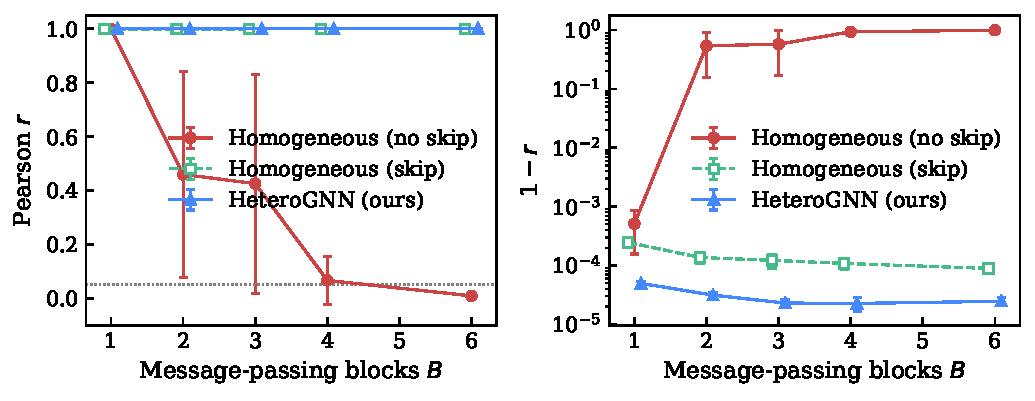
\includegraphics[width=\textwidth]{figures/depth_ablation.pdf}
\caption{Depth ablation at $16 \times 16$ (mean $\pm$ std over 3 seeds).
\textbf{Left:} Pearson $r$ vs.\ number of message-passing blocks $B$. The
homogeneous GNN without a readout skip connection degrades monotonically
with depth and collapses below $r = 0.05$ (dotted line) by $B = 6$; the
large error bars at $B = 2$--$3$ reflect bimodal seed-to-seed outcomes.
\textbf{Right:} $1 - r$ on a log scale, resolving the persistent gap between
the HeteroGNN and the skip-equipped homogeneous baseline at every depth.}
\label{fig:depth}
\end{figure*}

Beyond architectural stability, all spatially structured models achieve
$r > 0.99$, confirming that the $\phifour$ action is learnable as a local
functional. The HeteroGNN achieves the lowest relative error
($0.05\%$), roughly half that of the homogeneous GNN with its skip
connection ($0.11\%$). Matching the CNN's parameter count to the
HeteroGNN's (146k vs.\ 150k) narrows but does not close the gap: the
matched CNN reaches $r = 0.9995$ and $0.22\%$ relative error, a
$4\times$ larger error than the HeteroGNN at equal capacity, indicating
the advantage is architectural rather than a parameter-budget artifact.
The MLP baseline fails without any spatial structure ($r = 0.34$),
confirming that the lattice topology is essential. Seed-to-seed
variation is negligible for the graph models ($\sigma_r \lesssim 3
\times 10^{-5}$) and modest for the CNNs, so the ordering in
Table~\ref{tab:baselines} is stable.

\subsection{Coupling Generalization}
\label{sec:generalization}

To test whether the model learns a transferable action \emph{family} rather
than a single action landscape, the coupling constants are made model inputs:
field-node features become $[\phi_i, \msq, \lambda]$ and the readout MLP is
conditioned on $(\msq, \lambda)$ (adding 192 parameters). A single model is
then trained \emph{jointly} on alternating points of a 13-point $\msq$ grid
spanning $[-2.9, -0.3]$ at $\lambda = 0.5$ --- both phases and the critical
region --- with 3000 configurations per point (thermalization $\geq 2000$
sweeps; separations scaled by the measured $\tau_\text{int}$, up to 72 sweeps
near criticality). The held-out couplings interleave the training points
(interpolation test), and both grid endpoints are excluded from training
(extrapolation test).

In an earlier version of this experiment, a model trained at a single
coupling with no coupling input was evaluated against target actions computed
at each new $\msq$; since no function of $\phi$ alone can match a family of
action functionals indexed by a hidden parameter, that protocol measured a
partially unlearnable label shift on top of the distribution shift, and the
apparent degradation was severe (e.g.\ $r = 0.58$ at $\msq = -2.0$).
Table~\ref{tab:generalization} reports the corrected protocol.

\begin{table}[t]
\centering
\caption{Generalization across coupling values for a single
coupling-conditioned model trained jointly on the $\dagger$-marked $\msq$
points and evaluated on 1000 held-out configurations per coupling
($\ast$ = extrapolation beyond the training grid), over 5 seeds. We report $1 - r$ (smaller is better) since correlations are near unity; parenthetical uncertainties are seed-to-seed standard deviations. Relative error is inflated where the action distribution crosses
zero (near $\msq \approx -2.5$); Pearson $r$ is the meaningful metric
there.}
\label{tab:generalization}
% AUTO-GENERATED by scripts/make_paper_tables.py -- do not edit
\begin{tabular}{@{}lcc@{}}
\toprule
$\msq$ & $1 - r$ & Rel.\ Error \\
\midrule
$-2.9^\ast$ & $2.8(1.2) \times 10^{-3}$ & $19.52 \pm 2.65\%$ \\
$-2.6833^\dagger$ & $6.9(0.5) \times 10^{-6}$ & $0.07 \pm 0.00\%$ \\
$-2.4667$ & $5.2(1.0) \times 10^{-5}$ & $10.34 \pm 1.06\%$ \\
$-2.25^\dagger$ & $7.5(0.8) \times 10^{-6}$ & $5.58 \pm 0.75\%$ \\
$-2.0333$ & $6.4(0.9) \times 10^{-5}$ & $0.46 \pm 0.04\%$ \\
$-1.8167^\dagger$ & $1.8(0.1) \times 10^{-5}$ & $0.08 \pm 0.00\%$ \\
$-1.6$ & $2.3(0.2) \times 10^{-5}$ & $0.07 \pm 0.01\%$ \\
$-1.3833^\dagger$ & $1.7(0.1) \times 10^{-5}$ & $0.05 \pm 0.00\%$ \\
$-1.1667$ & $1.9(0.2) \times 10^{-5}$ & $0.06 \pm 0.01\%$ \\
$-0.95^\dagger$ & $1.4(0.1) \times 10^{-5}$ & $0.04 \pm 0.00\%$ \\
$-0.7333$ & $2.0(0.3) \times 10^{-5}$ & $0.08 \pm 0.03\%$ \\
$-0.5167^\dagger$ & $1.4(0.1) \times 10^{-5}$ & $0.04 \pm 0.00\%$ \\
$-0.3^\ast$ & $6.2(3.2) \times 10^{-5}$ & $0.55 \pm 0.34\%$ \\
\bottomrule
\end{tabular}

\end{table}

Table~\ref{tab:generalization} shows that with the couplings as inputs, the
single model interpolates essentially perfectly: every held-out interpolation
coupling reaches $r \geq 0.9999$, \emph{including} $\msq = -2.47$ in the
critical region where the old protocol appeared to fail. Extrapolation
beyond the training grid degrades only at the deep broken-phase endpoint
($\msq = -2.9$: $r = 0.9972 \pm 0.0012$), while the symmetric-phase endpoint
remains at $r = 0.9999$. Because the action is a strictly local functional
of the field, its prediction does not suffer near criticality once the label
family is identified --- long-range physics enters the ensemble
\emph{distribution}, not the action's functional form.

\subsection{Phase Transition and Finite-Size Scaling of the Training Ensembles}
\label{sec:fss}

This and the following subsection characterize the \emph{Monte Carlo
ensembles} used throughout this work: they validate the data-generation
pipeline against known Ising-universality results, rather than testing the
network itself. We map the phase transition of the two-dimensional \phifour\
theory at $\lambda = 0.5$ by a coupling sweep in \msq. Because the observables
of interest live at the critical point---exactly where the local Metropolis
update suffers critical slowing down---we generate the finite-size-scaling
ensembles with a Wolff/Brower--Tamayo embedded-cluster
sampler~\cite{Wolff1989,BrowerTamayo1989}: single-cluster $\mathbb{Z}_2$ sign
flips, whose dynamic exponent is $z \approx 0.25$ for this universality class,
interleaved with local sweeps that update the field magnitude. This holds the
integrated autocorrelation time to $\mathcal{O}(1)$ across the entire scan and
lets us reach $\Nsizes$ sizes up to $L = \Lmax$. We retain the local-Metropolis
ensembles at the same couplings as a direct measurement of the sampling bias
they carry.

\begin{figure*}[t]
\centering
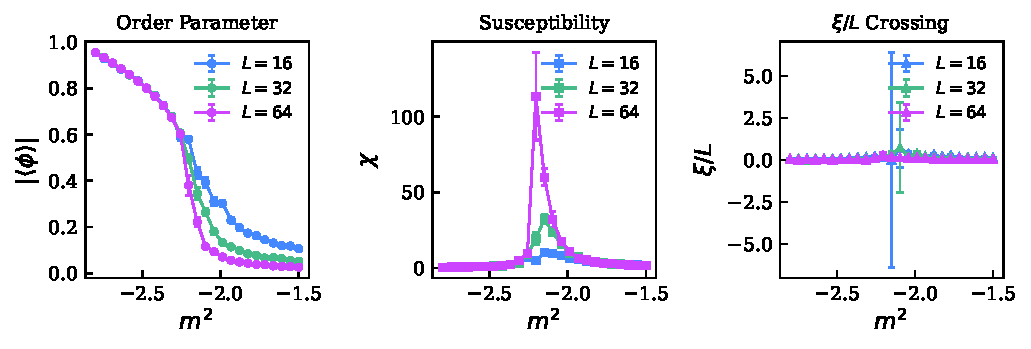
\includegraphics[width=\textwidth]{figures/finite_size_scaling.pdf}
\caption{Finite-size scaling of the cluster ensembles at $\lambda = 0.5$.
\textbf{Left:} order parameter $|M|$, sharpening with $L$. \textbf{Center:}
susceptibility $\chi$, with peaks growing as $\chi_\text{max} \sim
L^{\gamma/\nu}$. \textbf{Right:} correlation-length ratio $\xiL$, whose curves
cross near $\msqc = \ClMsqc$. Error bars are binned jackknife errors with bin
sizes set by the measured $\tau_\text{int}$; per-$L$ markers are
colorblind-distinct.}
\label{fig:fss}
\end{figure*}

Figure~\ref{fig:fss} shows the three canonical finite-size-scaling observables.
The qualitative picture---an order-parameter S-curve sharpening with $L$, a
growing susceptibility peak, and crossing $\xiL$ curves---is reproduced by both
samplers; the local ensembles, however, are quantitatively biased by critical
slowing down. Table~\ref{tab:tauint} lists the integrated autocorrelation time
of $|M|$ at each pseudocritical point in single sweeps: for the local update it
grows from $\TauLocLo$ at $L = 16$ to $\TauLocHi$ at $L = 64$ ($\tau \sim
\xi^z$, $z \approx 2$), while the cluster hybrid holds $\tau_\text{int} \approx
\TauClTyp$ independent of $L$---a decorrelation speed-up that reaches
$\SpeedupHi\times$ by $L = 64$ and makes $L = 96, 128$ practical at all.

The resulting bias in the exponent is direct. For the local ensembles the
effective slope of $\ln\chi_\text{max}$ versus $\ln L$ falls monotonically with
volume, from $\LocEffSlopeLo$ ($L = 16$--$24$) to $\LocEffSlopeHi$ ($L =
48$--$64$) as the largest lattices lose effective statistics, and a global fit
gives the downward-biased $\gamma/\nu = \LocGammaNu$. The cluster effective
slope shows no such trend. Locating the peaks by quadratic fits to dense scans
centered on each maximum (grid width $\propto L^{-1}$, so every fit spans the
same fraction of its peak and $\chi^2/\text{dof} \sim 1$), a weighted fit of
$\ln\chi_\text{max}$ versus $\ln L$ over all $\Nsizes$ sizes gives
\begin{equation}
\gamma/\nu = \ClGammaNu,
\label{eq:gammanu}
\end{equation}
consistent with the exact two-dimensional Ising value $\gamma/\nu = 1.75$. A
corrections-to-scaling fit $\chi_\text{max} = A\,L^{\gamma/\nu}(1 + b\,
L^{-\omega})$ with $\omega = 2$, and an Akaike-weighted average over
fit ranges~\cite{JayNeil2020}, give $\ClGammaNuCorr$ and $\ClGammaNuAIC$
respectively, consistent with the naive fit.

\begin{table}[t]
\centering
\caption{Susceptibility peak height $\chi_\text{max}$ and $|M|$ integrated
autocorrelation time (single sweeps, at the pseudocritical point) for the
local-Metropolis and cluster samplers. The local $\tau_\text{int}$ grows as
$\xi^z$ ($z \approx 2$); the cluster's stays $\mathcal{O}(1)$, and the local
sampler is impractical beyond $L = 64$ at these statistics.}
\label{tab:tauint}
\begin{tabular}{rccccc}
\toprule
& \multicolumn{2}{c}{$\chi_\text{max}$} & \multicolumn{2}{c}{$\tau_\text{int}(|M|)$} & \\
\cmidrule(lr){2-3}\cmidrule(lr){4-5}
$L$ & local & cluster & local & cluster & speed-up \\
\midrule
16 & 9.6(2) & 8.68(12) & 65 & 8.3 & 8 \\
24 & 18.7(6) & 18.2(2) & 104 & 12.8 & 8 \\
32 & 29.7(10) & 29.0(4) & 92 & 8.3 & 11 \\
48 & 56.5(18) & 58.9(7) & 141 & 8.6 & 16 \\
64 & 85(4) & 96.9(19) & 185 & 8.7 & 21 \\
96 & -- & 198(3) & -- & 8.7 & -- \\
128 & -- & 319(5) & -- & 8.7 & -- \\
\bottomrule
\end{tabular}

\end{table}

\subsection{Critical Exponent Extraction}
\label{sec:nu}

The correlation-length exponent and the critical coupling follow from the
approach of the pseudocritical points to the infinite-volume limit,
$\msq_\text{peak}(L) = \msqc - a\,L^{-1/\nu}$. A three-parameter fit to the
$\Nsizes$ cluster peak locations gives
\begin{equation}
\nu = \ClNu, \qquad \msqc = \ClMsqc \quad (\lambda = 0.5),
\label{eq:nu}
\end{equation}
with $\chi^2/\text{dof} = \ClNuChiDof$, consistent with the exact Ising $\nu =
1$. We quote this pseudocritical-shift fit rather than a $\xiL$ data collapse
because the naive collapse-quality metric has no proper interior minimum on
these data.\footnote{The same fit on the local ensembles gives $\nu = \LocNu$:
the central value agrees, but the local peak positions scatter under critical
slowing down ($\chi^2/\text{dof} \approx 4$), inflating the error roughly
sixfold.}

Two points frame these results. First, this is a validation of the training
ensembles, not a precision lattice study: dedicated determinations of the
two-dimensional \phifour\ critical line~\cite{SchaichLoinaz2009,DurrKiel2025}
reach far higher precision and use a different coupling normalization
(continuum-limit ratios $f = \lambda/\mu_c^2$ rather than a fixed bare $\lambda$
at finite spacing), so we do not attempt a quantitative comparison. Second---and
this is why we belabor the sampling---the exercise makes concrete the bottleneck
that motivates the broader program. The cluster algorithm that removes the bias
here exists only because the scalar theory has a simple $\mathbb{Z}_2$ order
parameter; no comparable algorithm is known for the gauge and fermion theories
targeted in the subsequent phases, where critical slowing down (and, with
dynamical fermions, the cost of the determinant) is the dominant obstacle to
generating training data. A learned surrogate for the action---the architecture
developed here---is one route into precisely that regime, where exact cluster
methods are unavailable.

\subsection{Size Transfer}
\label{sec:size-transfer}

The models above are trained one-per-lattice-size. To test whether a single
learned action functional transfers across volumes, we train at
$16 \times 16$ only and evaluate at $L \in \{8, 32, 64\}$ without any
retraining, for two spacetime-feature variants: absolute coordinates (as in
the rest of this paper) and a coordinate-free variant in which spacetime
nodes carry a constant feature and all geometry resides in the displacement
edge features (restoring exact translation invariance).

\begin{table}[t]
\centering
\caption{Size transfer: a single model trained at $16 \times 16$
($^\dagger$, validation split) evaluated at other lattice sizes without
retraining, over 3 seeds. We report $1 - r$ (smaller is better) since correlations are near unity; parenthetical uncertainties are seed-to-seed standard deviations.}
\label{tab:size-transfer}
% AUTO-GENERATED by scripts/make_paper_tables.py -- do not edit
\begin{tabular}{@{}lccc@{}}
\toprule
Variant & Eval.\ lattice & Pearson $r$ & Rel.\ Error \\
\midrule
Coordinates & $8 \times 8$ & $1.0000 \pm 10^{-6}$ & $0.10 \pm 0.00\%$ \\
 & $16 \times 16^\dagger$ & $1.0000 \pm 10^{-6}$ & $0.05 \pm 0.00\%$ \\
 & $32 \times 32$ & $1.0000 \pm 10^{-6}$ & $0.03 \pm 0.00\%$ \\
 & $64 \times 64$ & $1.0000 \pm 10^{-6}$ & $0.02 \pm 0.01\%$ \\
Coordinate-free & $8 \times 8$ & $1.0000 \pm 10^{-6}$ & $0.08 \pm 0.01\%$ \\
 & $16 \times 16^\dagger$ & $1.0000 \pm 10^{-6}$ & $0.04 \pm 0.00\%$ \\
 & $32 \times 32$ & $1.0000 \pm 10^{-6}$ & $0.02 \pm 0.00\%$ \\
 & $64 \times 64$ & $1.0000 \pm 10^{-6}$ & $0.01 \pm 0.00\%$ \\
\bottomrule
\end{tabular}

\end{table}

Table~\ref{tab:size-transfer} shows that the learned functional transfers
essentially perfectly in both directions --- down to $8 \times 8$ and up to
$64 \times 64$, a $64\times$ change in volume --- with $r = 1.0000$ at every
size for both variants. Relative error \emph{decreases} with lattice size
(from $0.10\%$ at $L=8$ to $0.01$--$0.02\%$ at $L=64$), consistent with an
accurate learned per-site action density whose fluctuations average out in
the extensive sum. The per-site readout (Eq.~\eqref{eq:action-readout}) is
what makes this possible: the same local functional applies at any volume.
Notably, even the absolute-coordinate variant transfers, indicating the
model learns to ignore the physically irrelevant coordinate inputs; the
coordinate-free variant is nevertheless preferable on principle (exact
translation invariance) and attains slightly lower relative error at every
size.

%=============================================================================
\section{Discussion}
\label{sec:discussion}
%=============================================================================

\subsection{Advantages of the Bipartite Architecture}

The heterogeneous bipartite graph offers several structural advantages over
homogeneous approaches:

\textbf{Multi-field extensibility.} In the homogeneous approach, adding a gauge
field $U_\mu(x) \in \text{SU}(N)$ requires concatenating its matrix elements
with the scalar field value at each node, breaking the natural group structure.
In our architecture, gauge fields become a separate node type with their own
encoder, connected to spacetime via typed edges. The three-stage message-passing
blocks handle arbitrary numbers of field types without modification.

\textbf{Physical interpretability.} The action readout
(Eq.~\eqref{eq:action-readout}) decomposes the total action into per-site
contributions $\hat{s}(x)$ that can be directly compared with the lattice
action density, enabling local error analysis.

\textbf{Metric information placement.}
\label{sec:metric-placement}
The lattice spacing $a$ is a metric quantity---it defines the physical distance
between neighboring sites. We encode it on adjacency edges as displacement
vectors $a\hat{e}_\mu$ rather than as a node feature, reflecting the fact that
distances are properties of connections, not of individual points. To validate
this choice, we tested four architecture variants (lattice spacing in
nodes vs.\ edges, with and without the explicit $a^d$ volume factor in
Eq.~\eqref{eq:action-readout}) across lattice sizes $8 \times 8$ through
$64 \times 64$ at varying lattice spacings $a = 1/L$. Two findings emerged.
First, the $a^d$ volume scaling is essential: without it, performance collapses
as $a$ decreases (Pearson $r$ drops from $>0.999$ to $-0.26$ at $64 \times 64$
with $a = 1/64$), because the MLP readout cannot learn to compensate for a
scale factor spanning four orders of magnitude. Second, the choice of whether
$a$ resides on nodes or edges has negligible effect on accuracy ($r > 0.999$
for both at all sizes), confirming that the placement is a design choice rather
than a performance constraint. We choose edges because the metric naturally
lives on links, and this design extends cleanly to gauge theories where link
variables $U_\mu(x)$ share the same edge representation.

\textbf{Over-smoothing mitigation.} By separating field and spacetime
representations, the architecture avoids mixing all information into a single
node type during message passing. Residual connections and layer normalization
further stabilize deep stacking.

\textbf{Interpretation as a learned effective action.} The action readout
(Eq.~\eqref{eq:action-readout}) decomposes the total action into per-site
contributions, and the finite receptive field of $B$ message-passing blocks
limits each contribution to information within $Ba$ lattice spacings. The model
therefore admits an interpretation as a \emph{local effective action}
operator---analogous to a Wilsonian effective action in which modes above a
momentum cutoff
$\Lambda \sim 1/(Ba)$ have been integrated out. In this view, the message-passing depth $B$ plays the role of an implicit
renormalization scale, controlling the resolution at which the theory is
represented. This interpretation explains both the model's success on the local
$\phifour$ action and its degradation near criticality, where the relevant
physics involves correlations at scales $\xi \gg Ba$ that lie below the
effective cutoff.

\subsection{Limitations}

\textbf{Critical slowing down.} The Metropolis sampler's autocorrelation time
diverges at the critical point, limiting our ability to precisely determine
$\nu$. This is a sampling limitation, not an architectural one.

\textbf{Receptive field and locality scale.} With $B = 3$ blocks, the model's
receptive field spans $\ell = Ba = 3a$, defining a finite \emph{locality scale}
for the learned operator. This is sufficient for the $\phifour$ action, which
is a strictly local functional of the field and its nearest-neighbor
differences --- and indeed action prediction remains accurate even at
couplings near criticality once the couplings are model inputs
(Sec.~\ref{sec:generalization}): the diverging correlation length changes the
ensemble \emph{distribution}, not the action's local functional form. The
locality scale becomes a genuine restriction for observables that are
themselves nonlocal --- correlators at separations $\gg \ell$, Wilson loops
of large area, or spectral quantities --- which the network cannot represent
regardless of coupling. Increasing $B$
enlarges the locality scale but risks over-smoothing, where distinct node
representations collapse toward a common value (measured directly in
Fig.~\ref{fig:depth} for the homogeneous baseline). For theories requiring
larger locality scales, possible mitigations include multi-scale pooling
layers, skip connections across non-adjacent blocks, or attention mechanisms
that allow selective long-range communication.

\textbf{Lattice symmetries.} The current architecture does not explicitly
enforce discrete lattice symmetries (translations, $C_4$ rotations,
reflections). Instead, these symmetries are learned implicitly from the data,
which is generated with periodic boundary conditions that respect the full
symmetry group. This is a deliberate design choice, not a limitation:
gauge-equivariant architectures~\cite{Favoni2022,Luo2021} --- including,
recently, gauge-equivariant message passing on graphs~\cite{Rayat2026} ---
achieve exact symmetry by constraining the network weights and message
functions, but this rigidity restricts them to the symmetry group built in
at design time. Our approach prioritizes \emph{architectural
flexibility}---the same model structure handles irregular meshes,
non-periodic boundaries, and adaptive lattice refinements without
modification. For the multi-theory extensibility that motivates this work
(gauge fields, fermions, curved spacetimes), this flexibility is essential.
Phase~II of this program (Sec.~\ref{sec:future}) will quantify the trade-off
directly by measuring the \emph{learned} gauge-invariance error of the
bipartite architecture against exactly equivariant designs such as
Ref.~\cite{Rayat2026}.

%=============================================================================
\section{Future Directions}
\label{sec:future}
%=============================================================================

The bipartite architecture is designed as a foundation for progressively more
complex theories:

\textbf{Phase~II: U(1) gauge theory with fermions.} Gauge link variables
$U_\mu(x) = e^{iA_\mu(x)} \in \text{U}(1)$ and Dirac spinors
$\psi(x) \in \mathbb{C}^2$ are added as new field node types with dedicated
encoders. The three-stage message passing naturally handles the tripartite
field--gauge--spacetime coupling. This phase will benchmark against the
Schwinger model (QED in 1+1D), which has exact solutions for comparison.

\textbf{Phase~III: SU(3) Yang--Mills in 4D.} In four dimensions, with link
encoders structured to respect the $\text{SU}(3)$ group, the target is to
reproduce established lattice QCD benchmarks such as the string tension and
glueball spectrum. Connecting the learned Euclidean representation to real-time
Minkowski physics is a longer-term and deliberately speculative direction.

%=============================================================================
\section{Conclusion}
\label{sec:conclusion}
%=============================================================================

The central result of this work is that representing lattice field theory as a
\emph{heterogeneous} graph---with spacetime geometry and field degrees of freedom
as distinct node types---eliminates a structural failure mode of the homogeneous
graph representations used previously, in which message passing destroys the
field signal without ad hoc skip connections. This geometry--field separation,
inspired by the geometry--matter distinction fundamental to continuum QFT and, to
our knowledge, absent from prior lattice-QFT neural
architectures~\cite{Favoni2022,Luo2021,Apte2024}, preserves a physically
interpretable local action decomposition. On two-dimensional scalar $\phifour$
theory, the model achieves near-perfect action prediction and transfers across a
$64\times$ range of lattice volumes without retraining; the underlying Monte
Carlo pipeline reproduces the expected Ising-class finite-size
scaling---$\gamma/\nu = \ClGammaNu$ and $\nu = \ClNu$, consistent with the exact
Ising values, once a cluster sampler removes the critical-slowing-down bias of
local updates---validating the ensembles the model is trained on. Comparison
against homogeneous GNN, CNN, and MLP baselines demonstrates the viability of the
bipartite representation for lattice field theory.

The architecture's key contribution is not improved accuracy on this benchmark
but its \emph{extensibility and physical alignment}: the same graph structure
and message-passing protocol accommodate scalar, gauge, and fermion fields
through modular encoder additions, while preserving the geometry--field
distinction throughout the computation. Metric information (lattice spacing) is
encoded on adjacency edges as displacement vectors, placing it where distances
physically reside and enabling clean integration with gauge link variables in
future phases. This provides a unified framework for progressing from toy models
to physically relevant theories, with lattice QCD as the ultimate target.

\ifanonymous
Code and data are available via an anonymized repository mirror (see the Data
availability section).
\else
Code and data are available at
\url{https://github.com/crosis19/qft-graph}.
\fi

\begin{acknowledgments}
% A pending acknowledgment awaits written permission -- see the note at the top
% of docs/schaich_email_draft.md (kept out of this file for review anonymity).
Generative AI was used in the preparation of this work. Anthropic's Claude
models (Claude Opus~4.6, Claude Opus~4.8, and Claude Fable~5, used via Claude
Code) assisted with implementing and testing the
simulation and analysis code, executing the finite-size-scaling analyses,
preparing figures, and drafting and editing portions of the manuscript. All
physics-critical code is covered by exact-value unit tests, every reported
number is regenerated from data in the public repository by committed scripts,
and all references were verified against the published records; the author
directed the work and takes full responsibility for its content.
Pre-submission feedback was obtained from OpenAI's ChatGPT (GPT-5.5) and
Google's Gemini (Gemini~3~Pro), which informed revisions to the presentation.

\ifanonymous
% Funding and conflicts-of-interest statements are omitted for double-anonymous
% review (a "no funding / independent" statement is itself identifying); they
% are declared in the cover letter and restored here on acceptance, per the
% IOP anonymisation checklist.
\else
This work received no funding from any agency in the public, commercial, or
not-for-profit sectors. The author declares no conflicts of interest.
\fi
\end{acknowledgments}

\section*{Data availability}
\ifanonymous
The analysis-level data supporting this study---Monte Carlo observables,
finite-size-scaling fit inputs and outputs, and training metrics---and all
code required to regenerate every figure, table, and quoted number are
available in an anonymized mirror of the project repository at
\url{https://anonymous.4open.science/r/qft-graph-3913} (identifying
information redacted for double-anonymous review; the public repository will
be linked on acceptance). Raw Monte Carlo field configurations and model
checkpoints are not deposited owing to their size, but are exactly
regenerable from the committed configuration files and seeds.
\else
The analysis-level data supporting this study---Monte Carlo observables,
finite-size-scaling fit inputs and outputs, and training metrics---and all
code required to regenerate every figure, table, and quoted number are openly
available at \url{https://github.com/crosis19/qft-graph}. Raw Monte Carlo
field configurations and model checkpoints are not deposited owing to their
size, but are exactly regenerable from the committed configuration files and
seeds.
\fi

\bibliography{references}

\end{document}
